\documentclass[a4paper, 11pt, titlepage]{article}
\setlength{\oddsidemargin}{0in} \setlength{\evensidemargin}{0in}
\setlength{\textwidth}{6.2in}
\setlength{\topmargin}{-0.2in} \setlength{\textheight}{8.8in}

\usepackage{graphicx}
\graphicspath{ {images/} }

\title{SE31520 Assignment 1 - Part 2: Forum for the CSA - version 1}
\author{Michal Wojciech Goly [mwg2]}
\date{30th November 2017}

\begin{document}

\maketitle
\tableofcontents
\newpage

\section{Introduction}
This document describes the architecture of the forum feature added to the CSA application
as part of the assignment submission for the SE31520 module at Aberystwyth University. The
following sections describe the design and implementation choices made during the development,
alongside testing performed and the implementation of the REST API. The report finishes with
the summary of the activities performed to achieve "flair" marks and sums up the work with
a critical evaluation.

\section{The CSA application}
I started the development by familiarising myself with the initial CSA architecture and
thinking about different ways I could add the forum functionality required. The Entity Relationship
Diagram below depicts the overall database schema of the final system, but my initial low fidelity
sketch included only the \texttt{Topics}, \texttt{Posts} and \texttt{Users} tables.

\subsection{Entity Relationship Diagram}
\begin{center}
  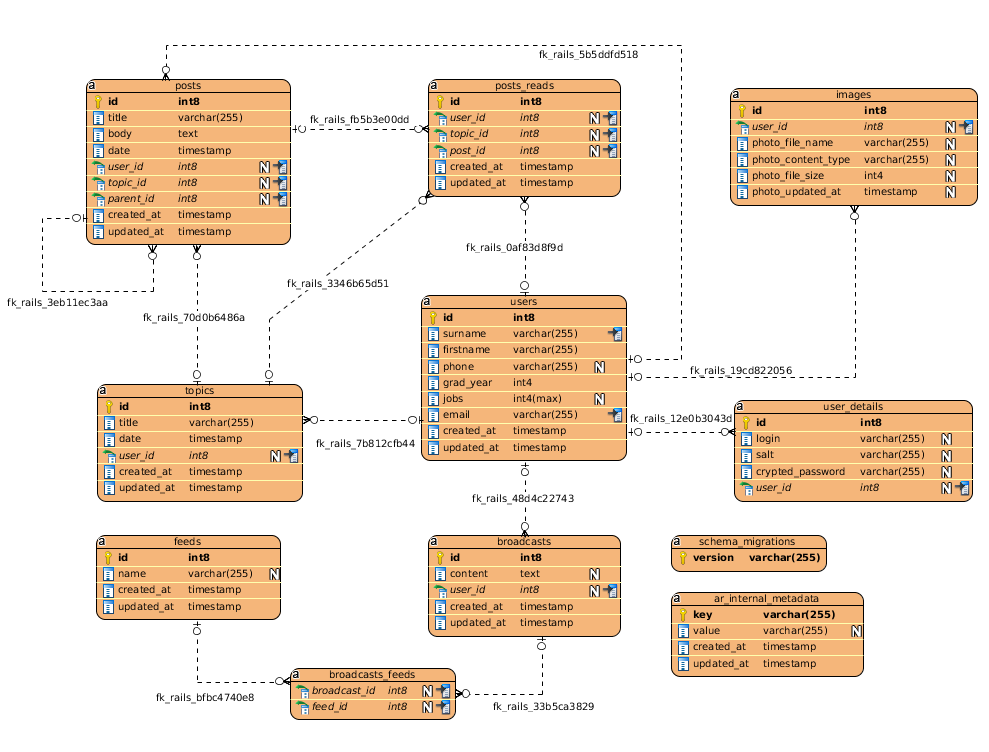
\includegraphics[scale=0.5]{schema}
\end{center}

\section{The REST client}

\section{Cucumber testing}

\section{Flair}
\subsection{The overall look and feel}
Materialize CSS

\subsection{Docker}
Docker and Docker Compose of test and dev environments

\subsection{Build and extra testing}
Circle CI, running integration, cucumber tests, deployment of master to a production environment

\subsection{Heroku}
link to the deployment env

\subsection{Feature branches and Kanban}
the development process, pull requests, screenshot of the kanban board

\section{Critical evaluation}
- Could have added controller tests, but did not know how to mock sessions in rails 5
- Improve the look and feel of the rest of the app

% \begin{thebibliography}{1}
%
% \bibitem{1} \emph{Active Record Basics}, guides.rubyonrails.org [Online],
% Available: http://guides.rubyonrails.org/active\_record\_basics.html, [Accessed: Oct. 22, 2017].
%
% \end{thebibliography}

\end{document}
